% Independent research materials. pdfLaTeX, two passes. No external figures.
\documentclass[aspectratio=169,10pt]{beamer}
\usepackage[english]{babel}
\usepackage[utf8]{inputenc}
\usepackage[T1]{fontenc}
\usepackage{lmodern,amsmath,booktabs,tabularx,array,tikz}
\usepackage{colortbl}
\usetikzlibrary{arrows.meta}
\usetheme{Madrid}
\definecolor{Ink}{HTML}{243748}
\definecolor{Muted}{HTML}{667B8B}
\definecolor{Accent}{HTML}{347E74}
\definecolor{AccentBlue}{HTML}{507DAD}
\definecolor{SoftMint}{HTML}{E6F4EE}
\definecolor{SoftLilac}{HTML}{F1EEF8}
\definecolor{Paper}{HTML}{FBFCFE}
\setbeamercolor{background canvas}{bg=Paper}
\setbeamercolor{normal text}{fg=Ink}
\setbeamercolor{structure}{fg=Accent}
\setbeamercolor{frametitle}{fg=Ink,bg=Paper}
\setbeamercolor{footline}{fg=Muted,bg=Paper}
\setbeamercolor{mintbox}{fg=Ink,bg=SoftMint}
\setbeamercolor{lilacbox}{fg=Ink,bg=SoftLilac}
\setbeamerfont{frametitle}{size=\large,series=\bfseries}
\setbeamertemplate{headline}{}
\setbeamertemplate{navigation symbols}{}
\setbeamertemplate{frametitle}{\nointerlineskip
\begin{beamercolorbox}[wd=\paperwidth,ht=.74cm,dp=.14cm,leftskip=.55cm]{frametitle}
\usebeamerfont{frametitle}\insertframetitle\end{beamercolorbox}}
\setbeamertemplate{footline}{\begin{beamercolorbox}[wd=\paperwidth,ht=.30cm,dp=.16cm,rightskip=.48cm]{footline}
\hfill\scriptsize Research Materials\enspace |\enspace\insertframenumber\,/\,\inserttotalframenumber\end{beamercolorbox}}
\setbeamersize{text margin left=.48cm,text margin right=.48cm}

\hypersetup{pdftitle={Research Direction \& Supporting Evidence},pdfauthor={Yu-Jui Liang}}
\newcommand{\srcA}{https://reellci.com/insights/the-hbf-inversion.html}
\newcommand{\srcB}{https://reellci.com/insights/hbm-footprint-inversion.html}
\newcommand{\srcC}{https://reellci.com/d/hbf-gen1-16hi/}
\newcommand{\srcD}{https://reellci.com/REEL\%20LCI\%20Methodology\%20Report\%20v1.0.pdf}
\newcommand{\srcE}{https://reellci.com/explorer/?category=memory_components}
\newcommand{\source}[1]{\vfill{\fontsize{6.8}{8}\selectfont\color{Muted}Source: #1\par}\vspace{.04cm}}
\newcommand{\takeaway}[1]{\par\vspace{.14cm}{\small\bfseries\color{Accent}#1\par}}
\newcommand{\card}[3]{\begin{beamercolorbox}[wd=\linewidth,rounded=true,sep=.17cm]{#1}
{\small\bfseries\color{Accent}#2}\par\vspace{.10cm}{\small\raggedright #3\par}\end{beamercolorbox}}
\newcommand{\researchquestion}[1]{\card{mintbox}{Research question}{#1}}
\tikzset{gridline/.style={draw=Muted!22},barHBM/.style={fill=AccentBlue},barHBF/.style={fill=Accent},chartlabel/.style={font=\scriptsize,align=center,text=Ink}}
% #1 = vertical unit scale; #2 = max; #3 = ticks; #4 = data; #5 = units
\newcommand{\carbonchart}[5]{%
\begin{tikzpicture}[x=1cm,y=#1cm]
\path[use as bounding box] (-.65,-#2*.24) rectangle (8.9,#2*1.18);
\node[anchor=west,font=\scriptsize,text=Muted] at (-.50,#2*1.13) {#5};
\foreach \y in {#3}{\draw[gridline] (0,\y)--(8.6,\y);\node[anchor=east,font=\scriptsize,text=Muted] at (-.12,\y){\y};}
\draw[Muted] (0,0)--(8.6,0);
\foreach \x/\v/\lab/\cap/\num/\sty in {#4}{
\path[\sty] (\x-.53,0) rectangle (\x+.53,\v);
\node[anchor=south,font=\small\bfseries,text=Ink] at (\x,\v+#2*.025){\num};
\node[chartlabel,anchor=north] at (\x,-#2*.035){\lab\\\cap};}
\end{tikzpicture}}
\begin{document}
\begin{frame}[plain,noframenumbering]
\vspace{.4cm}
{\small\bfseries\color{Accent}RESEARCH MATERIALS\par}
\vspace{.35cm}
{\LARGE\bfseries Research Direction\par\vspace{.10cm}\& Supporting Evidence\par}
\vspace{.30cm}
{\large HBM vs.\ HBF Embodied Carbon:\\Evidence and Comparison\par}
\vspace{.22cm}
{\color{Accent}\rule{2.2cm}{1.2pt}\par}
\vspace{.22cm}
{\large Yu-Jui Liang\quad Advisor: Hsiang-Yun Cheng\par}
\vspace{.12cm}
{\color{Muted}National Taiwan University / Academia Sinica\par}
\vspace{.24cm}
{\large Research Meeting\quad November 18, 2026\par}
\source{\href{\srcA}{REEL LCI v1.0: HBF comparison}; \href{\srcD}{Methodology report}. Model estimates, accessed 2026-11-13.}
\end{frame}

\begin{frame}[t]{What Evidence Do We Have for HBM/HBF Embodied Carbon?}
\vspace{.10cm}
\researchquestion{Can we obtain traceable manufacturing-carbon estimates for HBF before mass production?}
\vspace{.25cm}
\begin{columns}[T,onlytextwidth]
\begin{column}{.48\textwidth}
\card{mintbox}{REEL LCI v1.0}{Public semiconductor LCA methodology\\[5pt]
HBM3, HBM3E, HBM4 and HBF entries\\[5pt]
Fabrication and assembly assumptions\\[5pt]
Full inventory quantities require dataset access}
\end{column}
\begin{column}{.49\textwidth}
\card{lilacbox}{What this evidence supports}{A common framework for comparison\\[5pt]
A prospective HBF model without production data\\[5pt]
Preliminary sensitivity analysis\\[5pt]
Independent validation remains necessary}
\end{column}
\end{columns}
\vspace{.15cm}
\takeaway{A consistent starting point for embodied-carbon modeling,\\not verified HBF production measurements.}
\source{\href{\srcE}{REEL v1.0 dataset explorer}; \href{\srcC}{HBF dataset, quality and limitations}; \href{\srcD}{Methodology, Sec. 4.4.4 (PDF p. 68 / printed p. 66)}.}
\end{frame}

\begin{frame}[t]{How Much Embodied Carbon Does One Stack Carry?}
\relax
{\small\color{Muted}Published REEL LCI v1.0 screening estimates\par}
\vspace{.05cm}
\begin{columns}[c,onlytextwidth]
\begin{column}{.65\textwidth}
\carbonchart{.014}{250}{0,50,100,150,200,250}{1.2/13.52/{HBM3 8-Hi}/{16 GB}/13.52/barHBM,3.3/19.81/{HBM3 12-Hi}/{24 GB}/19.81/barHBM,5.4/20.6/{HBM3E 12-Hi}/{36 GB}/{\(\approx20.6\)}/barHBM,7.5/225.9/{HBF Gen 1}/{512 GiB}/225.9/barHBF}{kg CO$_2$e / stack}
\end{column}
\begin{column}{.32\textwidth}
\card{lilacbox}{HBF Gen 1, 16-Hi}{\LARGE\textbf{16.7$\times$}\par\vspace{.14cm}\small the per-stack carbon of HBM3 8-Hi\par\vspace{.20cm}
$225.9/13.52$\par\vspace{.20cm}
The HBF stack also offers substantially more capacity.}
\end{column}
\end{columns}
\takeaway{HBF has a substantially higher manufacturing-carbon cost per stack.}
{\scriptsize\color{Muted}Article estimates shown as published. Alignment with current detailed inventories has not been independently reproduced.\par}
\source{\href{\srcA}{HBF comparison, chart (13.52 / 19.81 / 225.9)}; \href{\srcB}{HBM comparison (20.6)}; \href{\srcE}{dataset capacity labels}. All model estimates, not manufacturer measurements.}
\end{frame}

\begin{frame}[t]{Does HBF Reduce Embodied Carbon per Unit Capacity?}
\relax
{\small\color{Muted}Nominal normalization: divide each published stack estimate by its capacity numeral\par}
\vspace{.05cm}
\begin{columns}[c,onlytextwidth]
\begin{column}{.65\textwidth}
\carbonchart{3.5}{1}{0,0.2,0.4,0.6,0.8,1.0}{1.2/.845/{HBM3 8-Hi}/{16 GB}/0.845/barHBM,3.3/.8254167/{HBM3 12-Hi}/{24 GB}/0.825/barHBM,5.4/.5722222/{HBM3E 12-Hi}/{36 GB}/{\(\approx0.572\)}/barHBM,7.5/.4412109/{HBF Gen 1}/{512 GiB}/0.441/barHBF}{kg CO$_2$e / nominal capacity unit}
\end{column}
\begin{column}{.32\textwidth}
\card{mintbox}{HBF vs. HBM3 8-Hi}{\LARGE\textbf{47.8\% lower}\par\vspace{.12cm}\small under nominal normalization\par\vspace{.16cm}
\footnotesize $1-\dfrac{225.9/512}{13.52/16}$\par\vspace{.16cm}\small
HBM labels: GB\\HBF label: GiB\\\textbf{Not a verified per-GiB comparison.}}
\end{column}
\end{columns}
\takeaway{HBF is lower after nominal capacity normalization, despite a higher stack cost.}
{\scriptsize\color{Muted}GB/GiB ambiguity remains. Lower carbon per capacity does not imply equal bandwidth, latency or serving performance.\par}
\source{\href{\srcA}{HBF comparison}; \href{\srcB}{HBM comparison}; \href{\srcE}{capacity labels}. Bars and 47.8\% are our calculations using unconverted capacity numerals.}
\end{frame}

\begin{frame}[t]{Can We Trust the HBF Carbon Estimate?}
\vspace{.10cm}
\begin{columns}[T,onlytextwidth]
\begin{column}{.49\textwidth}
\card{mintbox}{Current dataset assumptions}{\footnotesize
16-Hi stack, 512 GiB nominal capacity\\[6pt]
232-layer NAND + 65 nm CMOS proxy\\[6pt]
28 nm base logic, CBA bonding, TSV and testing\\[6pt]
175.6 mm$^2$ device envelope used as die area\\[6pt]
Assumed die yield: $\exp(-0.005\!\times\!175.6)\approx0.416$}
\end{column}
\begin{column}{.49\textwidth}
\card{lilacbox}{Limits that affect interpretation}{\footnotesize
No manufacturer production-carbon validation\\[6pt]
Package outline is not a measured die area\\[6pt]
Die area / bit density conflict remains unresolved\\[6pt]
Packaging and material inventory gaps\\[6pt]
Interposer, substrate and package assembly excluded}
\end{column}
\end{columns}
\vspace{.22cm}
{\small\textbf{Version caution:} Both the article and dataset say v1.0. The public inventory does not establish that today's assumptions reproduce 225.9 kg CO$_2$e.\par}
\vspace{.12cm}
{\footnotesize\color{Muted}The report gives a $-24\%/+32\%$ uncertainty band. We do not present it as a validated carbon interval around the article's estimate.\par}
\takeaway{Useful for scenarios. Independent validation is needed for definitive hardware-carbon claims.}
\source{\href{\srcC}{HBF dataset: assumptions, boundary and limitations}; \href{\srcD}{Methodology, Sec. 4.4.4, PDF p. 68 / printed p. 66}; \href{\srcA}{article estimate}.}
\end{frame}

\begin{frame}[t]{What Does This Mean for Our Research?}
\relax
{\small\bfseries\color{Accent}Power-Aware HBM/HBF Co-Design for Disaggregated MoE Serving\par}
{\footnotesize\color{Muted}Conceptual proposed architecture. No system-level carbon reduction demonstrated.\par}
\vspace{.06cm}
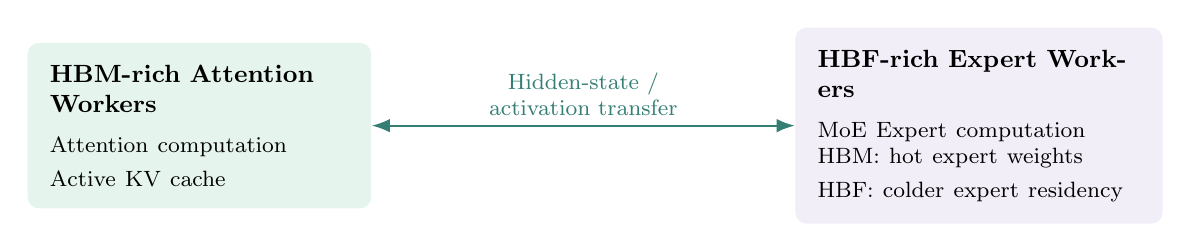
\begin{tikzpicture}[>=Latex]
\node[fill=SoftMint,rounded corners=4pt,inner sep=8pt,text width=3.8cm,minimum height=1.65cm,align=left] (a) at (2.2,0) {\small\textbf{HBM-rich Attention Workers}\\[5pt]\footnotesize Attention computation\\Active KV cache};
\node[fill=SoftLilac,rounded corners=4pt,inner sep=8pt,text width=4.1cm,minimum height=1.65cm,align=left] (e) at (12.1,0) {\small\textbf{HBF-rich Expert Workers}\\[5pt]\footnotesize MoE Expert computation\\HBM: hot expert weights\\HBF: colder expert residency};
\draw[<->,thick,Accent] (a.east)--(e.west) node[midway,above,align=center,font=\footnotesize]{Hidden-state /\\activation transfer};
\end{tikzpicture}
\vspace{.04cm}
{\centering\small\textbf{Total Carbon = Allocated Embodied Carbon + Operational Carbon}\par}
\vspace{.04cm}
{\footnotesize\textbf{Evaluate:} Memory configurations and GPU count; power and energy; TTFT / TPOT;\\goodput under SLO; HBF read stalls and communication overhead.\par}
\vspace{.05cm}
\researchquestion{Can heterogeneous HBM/HBF configurations reduce total LLM-serving carbon while meeting the same SLO constraints?}
\takeaway{The capacity-normalized estimate motivates evaluation, not a predetermined conclusion.}
\source{Architecture: our 2026-11-11 Research Direction (proposal). Carbon motivation: \href{\srcA}{REEL HBF comparison}; boundary: \href{\srcC}{HBF dataset}. Equation: proposed system accounting.}
\end{frame}
\end{document}
